\section{Intermediate Representations}
\label{bg:sec:intermediate}

Intermediate representations (IRs) are data structures designed to be
independent of the machine architecture and source language.  They are often
invented with the intention to ease program analysis and optimization in mind,
by abstracting information from the original program that are irrelevant to our
objectives.  In this section, we introduce several categories of existing IRs,
and delve deeper into the advantages and disadvantages of each.

\subsection{Static Single Assignment Form and Control-Flow Graph}
\label{bg:sub:ssa_cfg}

Traditionally, \emph{static single assignment} (SSA) form~\cite{alpern88,
rau92} together with \emph{control-flow graph} (CFG) are used to represent
data- and control-flow of a program~\cite{cytron91}, because they are more
favorable program representations on which optimization passes can be
implemented, when compared to the original HLL or the output language.  SSA can
be advantageous in implementing conventional optimization techniques, \eg~code
motion~\cite{cytron86}, removing redundant computations~\cite{rosen88},
and constant propagation~\cite{cytron91}.  Because the LLVM intermediate
representation (LLVM IR)~\cite{llvm_ir} is based on SSA and CFG, and is
commonly used in many HLS tools such as LegUp~\cite{legup}, we introduce SSA
and CFG by compiling the dot-product example in Figure~\ref{bg:lst:dotprod}
into as shown in Figure~\ref{bg:lst:dotprod_ll}.
\begin{figure}[ht]
    \centering
    \begin{lstlisting}[language=LLVM]
define float @dotprod(
    float* nocapture readonly %A,
    float* nocapture readonly %B) #0
{
; <label>:0
  br label %2

; <label>:1         ; preds = %2
  ret float %8

; <label>:2         ; preds = %2, %0
  %i.02 = phi i32 [ 0, %0 ], [ %9, %2 ]
  %d.01 = phi float [ 0.000000e+00, %0 ], [ %8, %2 ]
  %3 = getelementptr inbounds float, float* %A, i32 %i.02
  %4 = load float, float* %3, align 4, !tbaa !2
  %5 = getelementptr inbounds float, float* %B, i32 %i.02
  %6 = load float, float* %5, align 4, !tbaa !2
  %7 = fmul float %4, %6
  %8 = fadd float %d.01, %7
  %9 = add nuw nsw i32 %i.02, 1
  %exitcond = icmp eq i32 %9, 1024
  br i1 %exitcond, label %1, label %2
}
    \end{lstlisting}
    \caption{%
        The compiled and optimized LLVM IR output from the dot-product example
        in Figure~\ref{bg:lst:dotprod}.
    }\label{bg:lst:dotprod_ll}
\end{figure}

The LLVM IR of our example function consists of parts that are known as
\emph{basic blocks} (BB), each BB in turn often contains a label that
uniquely identifies the BB, a list of LLVM IR statements in SSA form
without any branches, \ie~the statements are executed sequentially, and a
terminator instruction, which is typically a branch instruction that leads
the control-flow to a different BB, by referencing a BB label, or a function
return.

The LLVM framework implicitly constructs a CFG from the IR code, which is a
directed graph representing the control-flow of a program.  The vertices in
the CFG constitute BBs, while the edges indicate the control-flow directions
(\ie~branches to other BBs), often with predicate attributes to determine
whether the branch is taken.  For instance, we consider the first line of third
BB in Figure~\ref{bg:lst:dotprod_ll}:
\begin{lstlisting}[language=LLVM, basicstyle=\tt]
    ; <label>:2     ; preds = %2 %0
\end{lstlisting}\vspace{-16.5pt}
which indicates it has a label value $2$ and the control-flow coming to this
BB is from either BB2 or BB0, here we use BB$n$ as a shorthand denoting a
BB labelled $n$.  Additionally, this BB ends with the branch terminator
instruction:
\begin{lstlisting}[language=LLVM, basicstyle=\tt]
    br i1 %exitcond, label %1, label %2
\end{lstlisting}\vspace{-16.5pt}
This instruction directs the control-flow to BB1 or BB2, and the variable
\verb|%exitcond| in the terminator instruction decides which branch is taken.
Finally, the complete CFG is shown in Figure~\ref{bg:fig:dotprod_cfg}.  It is
noteworthy that BB2 has two edges that leads to either \verb|BB1| or \verb|BB2|
itself.  If \verb|%exitcond| evaluates to false (\textbf{ff}), then another
iteration of BB2 will commence, otherwise (\textbf{tt}) the exit condition is
satisfied and will lead the control-flow to \verb|BB1|.
\begin{figure}[ht]
    \centering
    \tikzstyle{block} = [
        draw, fill=white, rectangle, minimum height=2em, minimum width=3em
    ]
    \tikzstyle{tmp} = [coordinate]
    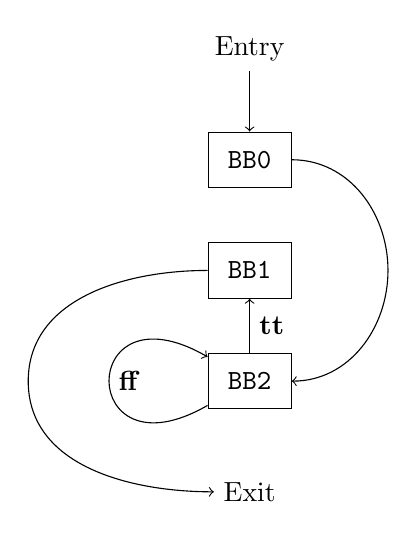
\begin{tikzpicture}
        \node [] (entry) {Entry};
        \node [block, below of=entry, node distance=4em] (bb0) {\texttt{BB0}};
        \node [block, below of=bb0, node distance=4em] (bb1) {\texttt{BB1}};
        \node [block, below of=bb1, node distance=4em] (bb2) {\texttt{BB2}};
        \node [tmp, right of=bb1, node distance=5em] (bb1tr) {};
        \node [tmp, left of=bb2, node distance=8em] (bb2tl) {};
        \node [tmp, right of=bb2, node distance=8em] (bb2tr) {};
        \node [below of=bb2, node distance=4em] (exit) {Exit};
        \draw [->] (entry) -- (bb0);
        \draw [- ] (bb0)    to[out=0, in=90]    (bb1tr);
        \draw [->] (bb1tr)  to[out=-90, in=0]   (bb2);
        \draw [- ] (bb1)    to[out=180, in=90]  (bb2tl);
        \draw [->] (bb2tl)  to[out=-90, in=180] (exit);
        \draw [->] (bb2) -- node[auto, swap]{\textbf{tt}} (bb1);
        \draw [->] (bb2) to[out=-150, in=150, loop]
            node[auto, swap]{\textbf{ff}} (bb2);
    \end{tikzpicture}
    \caption{The CFG of the LLVM IR code in Figure~\ref{bg:lst:dotprod_ll}.
    }\label{bg:fig:dotprod_cfg}
\end{figure}

Each BB contains sequential computations that are represented by SSA
instructions.  The SSA form describes the operations in the original
program, such that each variable in it is assigned exactly one value.

The sequence of instructions that assigns to \verb|%3|-\verb|%9| in
Figure~\ref{bg:lst:dotprod_ll} carries out most of the computations in the
program.  It starts by reading \verb|A[i]| and \verb|B[i]|, multiplying them
together, then add the result with \verb|d| to form a new variable, and
finally, the iteration value is accumulated by $1$.  It may seem unusual that
both the accumulated sum of products and the iteration value are not assigned
to \verb|d| and \verb|i| respectively.  We can imagine two BBs, one initializes
\verb|d| and \verb|i| to zeros, the other accumulates these two variables in
a loop.  As all variables must be assigned once only, one of the BBs should
use different names for these two variables.  When the control-flow of these
two BBs join, we must introduce a way to read from the variables that are
assigned in the two BBs in the succeeding BB\@.  A new instruction, called the
$\phi$-function is therefore defined for our purpose.  The $\phi$-function
accepts two variable names as its inputs, and produce the value of either
variable as its output, determined by which preceding BB the control-flow came
from.  For example, in LLVM IR, the instruction:
\begin{lstlisting}[language=LLVM, basicstyle=\tt]
    %d.01 = phi float [ 0.000000e+00, %0 ], [ %8, %2 ]
\end{lstlisting}\vspace{-16.5pt}
shows that if the control-flow originated from BB0, then a constant zero is
returned, otherwise the control-flow had to come from BB2 and the value of
\verb|%8| is used instead.

The rationale of SSA is that we can abstract away anti- and output dependences
by never assigning to the same variable twice, while only true data-flow
dependences remain.  Anti-dependence is a dependence relation when a read
operation must precede a write to the same variable, and output dependence is
when two writes refer to the same location.  By removing these two kinds of
dependences from the program representation, certain analyses on the program
to run much more efficiently.  Analyses that may benefit from this include
scheduling~\cite{rau94}, and liveness analysis (figure out the life time
of variables to reduce register requirements)~\cite{cytron91}, detecting
opportunities of parallelism~\cite{cytron87}, and finding equivalent parts in
the program~\cite{alpern88}.


\subsection{TODO}

\todo{Migrate old stuff from below.}
The structural optimization of general numerical programs is much more complex
than that of arithmetic expressions.  The reasons are two-fold.  First,
during program execution, variables are often updated with new values.  Our
optimization should therefore perform static analysis on the values of
variables, and use the result to optimize specifically for the trade-off
between accuracy and resource usage.  Second, it is much more difficult to
formally define program equivalence, and subsequently, to search efficiently
for optimized equivalent programs.  We proceed to explain further why this is
the case.

For instance, even without the introduction of branches and loops, the
following two programs in Figure~\ref{bg:fig:equiv_progs} are equivalent, but
syntactically, they are very different.
\begin{figure}[ht]
    \centering
    \subfloat[$P_1$]{%
        \shortstack[l]{%
            \texttt{x = x + 1;} \\
            \texttt{y = 2 * x;} \\
            \texttt{x = x + 3;}
        }
    } \qquad \qquad
    \subfloat[$P_2$]{%
        \shortstack[l]{%
            \texttt{y = x + 1;} \\
            \texttt{x = y;} \\
            \texttt{y = y * 2;} \\
            \texttt{x = x + 3;}
        }
    }
    \caption{%
        Two programs that are equivalent but syntactically different.
    }\label{bg:fig:equiv_progs}
\end{figure}

In fact, one can easily imagine infinitely many ways to rewrite numerical
programs, and often these equivalent programs have identical resource usage,
latency and accuracy characteristics.  In practice, it is desirable to
eliminate as much as possible the need for these syntactic rewrites that do not
affect our performance metrics, so that the search space of equivalent programs
is greatly reduced.

For this, we typically use an alternative representation of the original
program, which are called \emph{intermediate representations} (IRs).  These
representations include \emph{static} and \emph{dynamic single assignment
forms} (SSA, DSA)~\cite{rau92, cytron91}, and \emph{control and data flow
graphs} (CDFG)~\cite{gajski94}.  These IRs are however less suitable for
our work because they are all statement-based and do not identify as many
equivalent programs as MIRs do.  Dependence graphs~\cite{rau94}, on the other
hand, are designed for the purpose of capturing data-flow dependences in
polyhedral methods, but they generally do not preserve enough information for
us to reconstruct a program from the graph itself.

In software, \emph{equality saturation} is proposed in~\cite{tate09}.  It
creates a new intermediate representation, PEG, to encode the effects of
executing the program, and used to discover equivalent structures.  The
differences between PEG and what is required by us is that, instead of using
graphs with cycles in them to represent \whilelit~loops, we must use a
directed acyclic graph to encode programs and use a \emph{fixpoint} operator
to define recursive functions which can be used to represent loops.  Cycles in
graphs require reanalyzing a large proportion of the IR whenever a structural
modification is made, whereas a tree structure can be reasoned in a bottom-up
hierarchy.  This has significant implications on program transformation.
First, for the above reason, their approach does not use semantics to optimize
for numerical accuracy, while we want our method to reason about semantics
and utilize them to steer optimization.  Moreover, tree structure allows us
to easily support partial loop unrolling by simply extending the equivalence
relations while avoiding re-evaluation.  In contrast, like~\cite{martel09}
and~\cite{damouche15}, equality saturation is unable to perform partial loop
unrolling.
